\documentclass{article}

\usepackage{amsmath}
\usepackage{amssymb}
\usepackage{xcolor}
\usepackage{tikz}
\usepackage[shortlabels]{enumitem}
\usepackage{float}
\usepackage{wrapfig}

\usepackage[utf8]{inputenc}
\usepackage[T1]{fontenc}

\usepackage[polish]{babel}

\usepackage{listings}
\lstset{
    language=SQL,
    inputencoding=utf8x,
    extendedchars=\true,
    literate={ą}{{\k{a}}}1
             {Ą}{{\k{A}}}1
             {ę}{{\k{e}}}1
             {Ę}{{\k{E}}}1
             {ó}{{\'o}}1
             {Ó}{{\'O}}1
             {ś}{{\'s}}1
             {Ś}{{\'S}}1
             {ł}{{\l{}}}1
             {Ł}{{\L{}}}1
             {ż}{{\.z}}1
             {Ż}{{\.Z}}1
             {ź}{{\'z}}1
             {Ź}{{\'Z}}1
             {ć}{{\'c}}1
             {Ć}{{\'C}}1
             {ń}{{\'n}}1
             {Ń}{{\'N}}1
}

\title{Geometria analityczna}
\date{2026}

\begin{document}
\maketitle

\begin{enumerate}
%%%%%%%%%%%%%%%%%%%%%%%%%%%%%%%%%%%%%%%%%%%%%%%%%%%%%%%%%%%%%%%%%%%%%%%%%%%%%%%%%%%%%%%%%%%
\item Wyznaczyć współrzędne wktora w polarnym układzie współrzędnych:
    \begin{enumerate}[a)]
        \item $\begin{bmatrix} 1 & 1 \end{bmatrix} $,
        \item $\begin{bmatrix} -1 & 1 \end{bmatrix} $,
        \item $\begin{bmatrix} 0 & 1 \end{bmatrix} $,
        \item $\begin{bmatrix} -1 & -1 \end{bmatrix} $.
    \end{enumerate}

Współrzędne $(x,y)$ w kartezjańskim układzie współrzędnych można zapisać, zgodnie z rysunkiem (\ref{fig:pol}) jako:
$$
    (x,y) = (r\cos{\varphi}, r\sin{\varphi})
$$
\begin{figure}[H]\label{fig:pol}
    \centering
    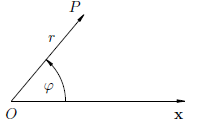
\includegraphics[width=0.5\linewidth]{fig/Przechwytywanie.PNG}
    \caption{Polarne współrzędne.}
    \label{fig:enter-label}
\end{figure}
Zatem zapis $(x,y)$ jest równoważny zapisowi $(r,\varphi)$ - długość wektora i kąt między osią $X$ -  gdyż jednoznacznie opisuje on punkt na płaszczyźnie (z wyjątkiem punktu $(0,0)$, dla którego nie można jednoznacznie podać kąta $\varphi$).

Zatem aby z układu kartezjańskiego przejść na polarny należy wyznaczyć $r$ i $\varphi$:
$$
    r = \sqrt{x^2 + y^2}, \, \varphi = \arctan{\frac{y}{x}}
$$

Dla przykładu a) będzie to:
$$
    r = \sqrt{1^2 + 1^2} = \sqrt{2}, \varphi = \arctan{\frac{1}{1}} = \frac{\pi}{4}
$$

%%%%%%%%%%%%%%%%%%%%%%%%%%%%%%%%%%%%%%%%%%%%%%%%%%%%%%%%%%%%%%%%%%%%%%%%%%%%%%%%%%%
\item Wyznaczyć współrzędne wektora w sferycznym układzie współrzędnych:
    \begin{enumerate}[a)]
        \item $\begin{bmatrix} 1 & 1 & 1 \end{bmatrix} $,
        \item $\begin{bmatrix} -1 & 1 & 0 \end{bmatrix} $,
        \item $\begin{bmatrix} 0 & 1 & 0 \end{bmatrix} $,
        \item $\begin{bmatrix} 0 & 0 & 1 \end{bmatrix} $.
    \end{enumerate}

Współrzędne $(x,y,z)$ w kartezjańskim układzie współrzędnych można zapisać, zgodnie z rysunkiem (\ref{fig:sfer}) jako:
$$
    (x,y,z) = (r\cos{\varphi}\cos{\theta}, r\sin{\varphi}\cos{\theta}, r\sin{\theta})
$$
\begin{figure}[H]\label{fig:sfer}
    \centering
    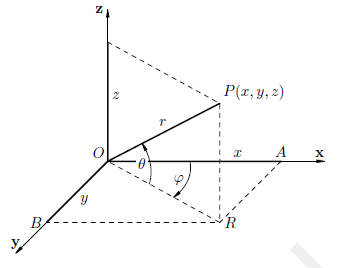
\includegraphics[width=0.5\linewidth]{fig/Przechwytywanie2.PNG}
    \caption{Sferyczne współrzędne.}
    \label{fig:enter-label}
\end{figure}
Zatem zapis $(x,y,z)$ jest równoważny zapisowi $(r,\varphi,\theta)$ - gdyż jednoznacznie opisuje on punkt na płaszczyźnie (z wyjątkiem punktu $(0,0, z)$, dla którego nie można jednoznacznie podać kąta $\varphi$ i).

Zatem aby z układu kartezjańskiego przejść na polarny należy wyznaczyć $r$, $\varphi$ i $\theta$:
$$
    r = \sqrt{x^2 + y^2 + z^{2}}, \, \varphi = \arctan{\frac{y}{x}}, \, \theta = \arcsin{\frac{z}{\sqrt{x^2 + y^2 + z^{2}}}}
$$

Dla przykładu a) będzie to:
$$
    r = \sqrt{1^2 + 1^2 + 1^2} = \sqrt{3}, \varphi = \arctan{\frac{1}{1}} = \frac{\pi}{4}, \, \theta = \arcsin{\frac{1}{\sqrt{1^2 + 1^2 + 1^2}}} \approx 0.6155
$$
%%%%%%%%%%%%%%%%%%%%%%%%%%%%%%%%%%%%%%%%%%%%%%%%%%%%%%%%%%%%%%%%%%%%%%%%%%%%%%%%%%%%%%
\item Wyznaczyć równanie kierunkowe prostej na płaszczyźnie na podstawie równania ogólnego:
    \begin{enumerate}[a)]
        \item $x + y + 1 = 0$,
        \item $2x - y + 2 = 0$,
        \item $y + 2 = 0$,
        \item $x + 1 = 0$.
    \end{enumerate}

    Równianie ogólne prostej ma postać:
    $$
        Ax + By + C = 0
    $$
    Równanie kierunkowe prostej ma postać:
    $$
        y = ax + b
    $$
    Łatwo zauważyć, że w sytuacji gdy $B \neq 0$ można wyznaczyć równanie kierunkowe w postaci:
    $$
        x = -\frac{A}{B}x - \frac{C}{B} = ax + b
    $$
    gdzie $a = -\frac{A}{B}$ i $b = -\frac{C}{B}$

    Zatem dla przykładu a) mamy:
    $$
        y = -x - 1
    $$

%%%%%%%%%%%%%%%%%%%%%%%%%%%%%%%%%%%%%%%%%%%%%%%%%%%%%%%%%%%%%%%%%%%%%%%%%%%%%%%%%%%%%%
\item Wyznaczyć równanie parametryczne prostej przechodzącej przez punkty:
    \begin{enumerate}[a)]
        \item $P_{0} = (1,1), \, P_{1} = (0,0)$,
        \item $P_{0} = (1,2), \, P_{1} = (1,0)$,
        \item $P_{0} = (1,1,1), \, P_{1} = (0,1,3)$,
        \item $P_{0} = (1,1,0), \, P_{1} = (2,0,4)$.
    \end{enumerate}

Równanie parametryczne prostej ma postać:
$$
    r = r_{0} + vt
$$
gdzie $t$ jest parametrem. Interpretacja graficzna przedstawiona jest na rysunku (\ref{fig:param})
\begin{figure}[H]\label{fig:param}
    \centering
    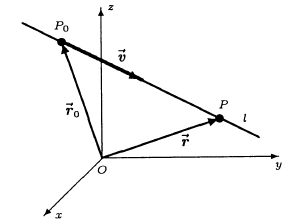
\includegraphics[width=0.5\linewidth]{fig/Przechwytywanie3.PNG}
    \caption{Równanie parametryczne prostej}
    \label{fig:enter-label}
\end{figure}
Na podstawie rysunku łatwo zauważyć, że wektor $v$ można wyznaczyć przez odejmowanie $P_{1} - P_{0}$.
Natomiast $r_{0}$ jest dowolnym punktem z tej prostej - najłatwiej przyjać $r_{0} = P_{0}$.

Dla przykładu a) mamy $v = P_{1} - P_{0} = (0,0) - (1,1) = (-1, -1)$, oraz $r_{0} = P_{0} = (1,1)$.
Zatem równanie ma postać:
$$
    r = (1,1) + (-1,-1)t
$$
Bądź w formie rozpisanej:
$$
    \left\{
    \begin{array}{l}
        x = x_{0} - v_{x}t = 1 - t  \\
         y = y_{0} - v_{y}t = 1 - t
    \end{array}
    \right.
$$


%%%%%%%%%%%%%%%%%%%%%%%%%%%%%%%%%%%%%%%%%%%%%%%%%%%%%%%%%%%%%%%%%%%%%%%%%%%%%%%%%%%%%%
\item Wyznaczyć równanie ogólne prostej przechodzącej przez punkt $P_{0} = (x_{0},y_{0})$ prostopadłej do wektora $u = (A,B)$:
    \begin{enumerate}[a)]
        \item $P_{0} = (1,1), \, u = (1,1)$,
        \item $P_{0} = (1,2), \, u = (1,0)$,
        \item $P_{0} = (1,1), \, u = (0,1)$,
        \item $P_{0} = (1,1), \, u = (2,0)$.
    \end{enumerate}

Można zauważyć, że prosta prostopadła do wektora $u=(A,B)$ ma postać:
$$
    Ax + By + C = 0
$$
\begin{figure}[H]\label{fig:zad5}
    \centering
    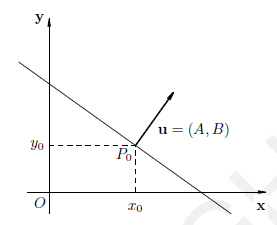
\includegraphics[width=0.5\linewidth]{fig/Przechwytywanie4.PNG}
    \caption{Prosta prostopadła do wektora $u=(A,B)$.}
    \label{fig:enter-label}
\end{figure}
Aby prosta przechodziła dodatkow przez punkt $P_{0} = (x_{0},y_{0})$ ma ona postać:
$$
    A(x-x_{0}) + B(y-y_{0}) = 0
$$

Dla przykładu a) jest to: $A = 1$, $B=1$, $x_{0} = 1$ i $y_{0} = 1$, zatem:
$$
    A(x-x_{0}) + B(y-y_{0}) = Ax - Ax_{0} + By - By_{0} = x + y -2 = 0
$$

%%%%%%%%%%%%%%%%%%%%%%%%%%%%%%%%%%%%%%%%%%%%%%%%%%%%%%%%%%%%%%%%%%%%%%%%%%%%%%%%%%%%%%
\item Wykonać ortogonalizację bazy:
    \begin{enumerate}[a)]
        \item $b_{1} = (2,0),\,b_{2} = (1, 1)$,
        \item $b_{1} = (1,2),\,b_{2} = (0, 1)$,
        \item $b_{1} = (1,0,1),\,b_{2} = (0, 1, 0),\,b_{3} = (0, 0, 1)$,
        \item $b_{1} = (1,1,1),\,b_{2} = (1, 1, 0),\,b_{3} = (1, 0, 0)$.
    \end{enumerate}

Ortogonalizacj bazy $b_{1}, \cdots, b_{n}$ do bazy ortogonalnej $u_{1}, \cdots, u_{n}$ można dokonać metodą Grama-Schmidta. Metoda ta ma następujący algorytm:
\begin{itemize}
    \item $u_{1} := b_{1}$ - pierwszy wektor bazy bez zmian,
    \item $u_{2} := b_{1} - \pi_{u_{1}}(b_{2})$ - rzut prostokątny wektora $b_{2}$ na prostą wyznaczaną przez wektor $b_{1}$,
    \item $\vdots$
    \item $u_{n} := b_{n} - \pi_{span\{u_{1}, \cdots, u_{n-1}\}}(b_{n})$ - rzut prostokątny na podprzestrzeń wyznaczaną przez wektory nowej bazy, od $1$ do $n-1$.
\end{itemize}
Graficzna reprezentacja jest przedstawiona poniżej.
\begin{figure}[H]\label{fig:ogs}
    \centering
    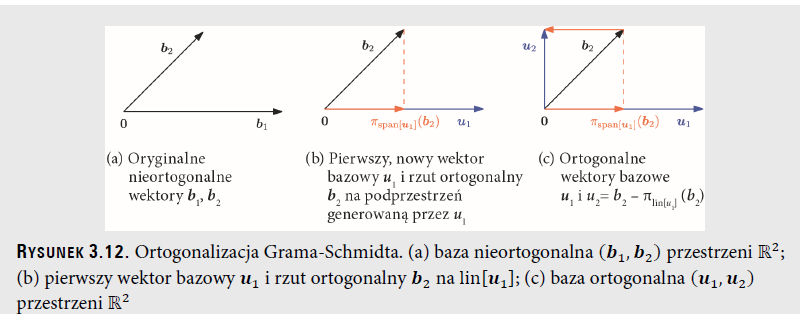
\includegraphics[width=1.0\linewidth]{fig/Przechwytywanie5.PNG}
    \caption{Ortogonalizacja Grama-Scmidta.}
    \label{fig:enter-label}
\end{figure}
Aby uzyskać bazę ortonormalną wystarczy wykonać: $u_{i} := \frac{u_{i}}{||u_{i}||},\forall{i}$.

Dla przykładu a) mamy:
\begin{itemize}
    \item $u_{1} := b_{1} = \begin{bmatrix}\begin{array}{r} 2\\ 0 \end{array}\end{bmatrix}$,
    \item $u_{2} := b_{2} - \pi_{u_{1}}(b_{2}) = b_{2} - \frac{u_{1}u_{1}^{T}}{u_{1}^{T}u_{1}}b_{2} = \begin{bmatrix}\begin{array}{r} 1\\ 1 \end{array}\end{bmatrix} - \begin{bmatrix}\begin{array}{rr} 1&0\\ 0&0 \end{array}\end{bmatrix} \begin{bmatrix}\begin{array}{r} 1\\ 1 \end{array}\end{bmatrix} = \begin{bmatrix}\begin{array}{r} 0\\ 1 \end{array}\end{bmatrix}$,
\end{itemize}

%%%%%%%%%%%%%%%%%%%%%%%%%%%%%%%%%%%%%%%%%%%%%%%%%%%%%%%%%%%%%%%%%%%%%%%%%%%%%%%%%%%%%%
\item Wyznaczyć równanie ogólne płaszczyzny przechodzącej przez punkty:
    \begin{enumerate}[a)]
        \item $P_{0} = (1,1,1), \, P_{1} = (0,0,0), P_{2} = (1,2,1)$,
        \item $P_{0} = (1,0,1), \, P_{1} = (0,1,0), P_{2} = (2,2,0)$,
        \item $P_{0} = (0,1,1), \, P_{1} = (1,0,0), P_{2} = (1,2,0)$,
        \item $P_{0} = (1,1,0), \, P_{1} = (0,0,2), P_{2} = (1,2,1)$.
    \end{enumerate}
Równanie ogólne płasczyzny ma postać:
$$
    Ax + By + Cz + D = 0
$$
Analogicznie jak w przypadku prostej, można zauważyć, że wektory rozpinające tą płaszczyznę są ortogonalne do wektora normnalnego płaszczyzny $n = (A, B, C)$.
\begin{figure}[H]\label{fig:fff}
    \centering
    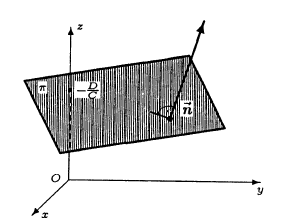
\includegraphics[width=0.5\linewidth]{fig/Przechwytywanie6.PNG}
    \caption{Płaszczyzna i wektor normalny.}
    \label{fig:enter-label}
\end{figure}
Można zauważyć, że jeśi płasczyzna ma przechodzić przez 3 punkty (nie leżące na jednej prostej), to zawiera ona dwa wektory $P_{0}P_{1}$ oraz $P_{0}P_{2}$.
Na ich podstawi można znaleźć wektor normalny - znajdując wektor ortogonalny do obydwu, a to można osiągnać wyznaczając iloczyn wktorowy tych wektorów:
$$
    n
    =
    \begin{vmatrix}\begin{array}{rrr}
        \hat{i} & \hat{j} & \hat{k}\\
        x_{0}  & y_{0} & z_{0}\\
        x_{1}  & y_{1} & z_{1}
    \end{array}\end{vmatrix}
$$

Dla przykładu a) mamy
$$
    v_{1} = P_{0} - P_{1} = (1,1,1) - (0,0,0) = (1, 1,1),\,
    v_{2} = P_{0} - P_{2} = (1,1,1) - (1,2,1) = (0,-1,0),
$$
Z tego wyznaczmy wektor normalny:
$$
    n = v_{1} \times v_{2} =
    \begin{vmatrix}\begin{array}{rrr}
        \hat{i} & \hat{j} & \hat{k}\\
        1  & 1 & 1\\
        0  & -1 & 0
    \end{array}\end{vmatrix}
    = -\hat{i} + \hat{k} = (-1,0,1)
$$
Zatem równanie płaszczyzny ma postać:
$$
    -(x-x_{0}) + (z-z_{0}) = -x+y + x_{0}-z_{0} = -x+y=0
$$
\end{enumerate}

\end{document}